请注意\eqref{eq:4-electron-interaction-by-phonon}实际上是做了近似的,因为声子的传播速度有限,因此把声子积掉之后得到的任何相互作用必然是一个推迟相互作用,而\eqref{eq:4-electron-interaction-by-phonon}给出的相互作用是瞬时的。%
\footnote{
    实际上我们甚至可以大致确定推迟相互作用的形式。$\omega_{\vb*{q}}$是声子能量,它不太可能和推迟有关,因为推迟应当是“某个关于电子的能量量纲的量乘以电子场的时间”,即$\exp(\ii \epsilon_{\vb*{k}} \tau)$。
    电子能量的绝对大小无关紧要,同样不会直接决定推迟,那么唯一能够决定推迟时间的时间尺度的只能是
    \[
        \omega = \epsilon_{\vb*{k}} - \epsilon_{\vb*{k} + \vb*{q}}.
    \]
    这样,设推迟相互作用的作用量为
    \[
        S \sim D \bar{c}(\vb*{k}+\vb*{q}, \tau) \bar{c}(\vb*{k}'-\vb*{q}, \tau') c(\vb*{k}, \tau) c(\vb*{k}', \tau'),
    \]
    则
    \[
        D \sim \sum \abs{M_{\vb*{q}}}^2 \frac{\omega_{\vb*{q}}}{\omega^2 - \omega_{\vb*{q}}^2} \ee^{\omega(\tau - \tau')}.
    \]
    这是为了保证$\tau=\tau'$时回退到\eqref{eq:4-electron-interaction-by-phonon}。这样,对\eqref{eq:4-electron-interaction-by-phonon}中的相互作用强度以$\omega$为变量做傅里叶变换就能够大致知道推迟相互作用的形式。

    当然,实际上以上推导仅仅表明推迟相互作用在推迟不大时可以回退到\eqref{eq:4-electron-interaction-by-phonon},并不能够严格说明\eqref{eq:4-electron-interaction-by-phonon}一定来自一个推迟相互作用。我们归根到底还是通过声子的性质来确定相互作用确实是推迟的这一事实的,\eqref{eq:4-electron-interaction-by-phonon}中有$\omega$依赖只是一个暗示。
}%

%%%%%%%%%%%%%%%%%%%%%%%%%%%%%%%%%%%%%%%%%%%%%%%%%%%%%%%%%%%%%5

\subsubsection{费米液体}

朗道注意到,很多相互作用电子气的行为和自由电子气实际上非常相似,参数可能不同但是定性行为都是一样的。
这是因为对自由电子气系统,我们可以浸染地将相互作用加入,如果相互作用强度较小,这只会带来电子的自能修正和一个势能项,因为如果相互作用很小,那么可以以自由电子气系统的能量本征态为零级波函数,计算相互作用带来的一阶修正,相互作用仅仅会把自由电子气系统的能量本征态旋转一个小角度,不会改变本征态的结构。
这样的近独立“电子气”称为\concept{费米液体}。%
\footnote{由于从气体到液体的相变没有出现任何对称性破缺,应当使用完全一样的哈密顿量来描写气体和液体。于是我们将粒子间相互作用弱的系统称为气体,将有强关联但是还没有出现晶格的系统称为液体。}%
如果相互作用较强,虽然加入相互作用之后表面上理论还是加了自能修正的电子气,但是能标较低时就可能出现相变。

费米液体中的“电子”实际上并不是电子——想象一个电子在实际的电子气的费米面外面运动,由于相互作用,会“激起一片涟漪”,这样导致的一系列电子的集体运动模式就是准粒子,费米液体中的粒子实为这种准粒子。
由于相互作用等价于加入了自能修正,准粒子的自旋没有发生变化,但是质量发生了变化,且格林函数中会出现一个明显的虚部,即粒子寿命有限。
然而,我们还是可以从费米液体中准粒子的行为中看到很明显的裸电子的影子:例如,准粒子的个数和电子的个数是一样的,准粒子的能谱的形式和电子的能谱很相似,等等。

当然,费米液体的图像并不适用于任意的体系,比如说如果电子相互作用造成某种配对,那么显然最后形成的准粒子个数是电子个数的一半,而且能谱的形式也大不相同。

通常准粒子的寿命在接近费米面时比较长,因此看起来像是“真正的”粒子(否则会有非常明显的能级展宽)。
这件事的原因如下。设准粒子寿命为$\tau$,则$\tau$反比于散射率,而散射率正比于库仑相互作用的强度。完整地做这个计算是很困难的,因为涉及到静电屏蔽等复杂的效应。
由于我们只做数量级估计,暂时将寿命对整个费米面做平均,从而使用一个常数$M$表示相互作用强度。
散射的过程可以概括为:一个动量为$\vb*{p}$的费米面外部的电子(实际上是费米液体中的准粒子,下同)的能量降低,变成了动量为$\vb*{p}_1$的电子,同时激发了一个费米面内的动量为$\vb*{p}_2$的电子。
结果是,动量为$\vb*{p}$的费米面以外的电子衰变成了两个电子,动量分别为$\vb*{p}_1$和$\vb*{p} - \vb*{p}_1 + \vb*{p}_2$,还有一个动量为$\vb*{p}_2$的空穴。
设动量分别为$\vb*{p}_1$和$\vb*{p} - \vb*{p}_1 + \vb*{p}_2$的两个电子和动量为$\vb*{p}_2$的空穴的总态密度在当前温度下的期望值为$n$,由费米黄金法则有
\[
    \frac{1}{\tau} \propto \text{transition rate} \sim \abs{M}^2 n.
\]
由于系统中的电子非常多,不同能级上电子数的涨落可以略去,即认为不同能级上不多不少正好就有费米-狄拉克分布\eqref{eq:fermi-dirac-distribution}给出的电子个数,%
\footnote{这是热力学系统的一般性质:系统规模大时涨落可略去。由于本文涉及的系统都是多体系统,总是可以做这样的近似。}%
那么就有
\[
    n = \int \dd[3]{\vb*{p}_1} \int \dd[3]{\vb*{p}_2} (1 - f(\epsilon_{\vb*{p}_1})) f(\epsilon_{\vb*{p}_2}) (1 - f(\epsilon_{\vb*{p} - \vb*{p}_1 + \vb*{p}_2})) \delta(\epsilon_{\vb*{p}} - \epsilon_{\vb*{p}_1} + \epsilon_{\vb*{p}_2} - \epsilon_{\vb*{p} - \vb*{p}_1 + \vb*{p}_2}).
\]
因子$(1-\epsilon_{\vb*{p}_1})$表示动量为$\vb*{p}_1$的电子应该占据一个空态(或者说在接近零温时应该在费米面以外),因子$f(\epsilon_{\vb*{p}_2})$表示空穴一定来自一个已有的电子,最后的$\delta$函数强制要求能量守恒。
我们不严格计算这个积分,而是做一些数量级估计。
由于$\vb*{p}_2$在费米面以下而$\vb*{p}- \vb*{p}_1 + \vb*{p}_2$在费米面以上,容易写出以下不等式
\[
    0 < \xi_{\vb*{p}_1} < \xi_{\vb*{p}}, \quad 0 < - \xi_{\vb*{p}_2} < \xi_{\vb*{p}} - \xi_{\vb*{p}_1} < \xi_{\vb*{p}},
\]
对$n$有贡献的$\vb*{p}_1$和$\vb*{p}_2$均满足这些不等式,这些不等式给出了两个宽度为$\xi_{\vb*{p}}$的球壳,因此
\[
    n \leq (4 \pi k_\text{F}^2 \xi_{\vb*{p}})^2,
\]
于是
\begin{equation}
    \frac{1}{\tau} \lesssim \xi_{\vb*{p}}^2.
\end{equation}
因此,如果准粒子非常接近费米液体的费米面,那么它是非常稳定的,因为此时$\xi_{\vb*{p}}$很小。从物理图像上看,此时的准粒子虽然会和费米海中的准粒子发生相互作用,但其能量不足以产生电子-空穴对,因此也不会衰变。

通常只分析费米面附近的物理,部分原因在于只有这里才确定有稳定的准粒子,部分原因在于费米海的结构可以非常复杂,因此只考虑费米面附近的物理是比较容易的,也是比较有实际意义的。
考虑一个能量本征态,其中准粒子在费米面之上的数量为$\var{n}$,则总是把能量本征值相对于零温平衡态(由于费米海的结构可以非常复杂,平衡态能量反而是算不出来的)的变化写成以下级数展开($\vb*{k}$在费米面附近):
\begin{equation}
    \var{E} = \underbrace{\sum_{\vb*{k}, \sigma} \epsilon^0_{\vb*{k}} \var{n_{\vb*{k} \sigma}}}_{\var{E_1}} + \underbrace{\frac{1}{2V} \sum_{\vb*{k}, \vb*{k}', \sigma, \sigma'} f_{\sigma \sigma' \vb*{k} \vb*{k}'} \var{n_{\vb*{k} \sigma}} \var{n_{\vb*{k}' \sigma'}}}_{\var{E_2}},
    \label{eq:fermi-liquid-energy}
\end{equation}
其中$\var{n}$表示准粒子数目相对基态的变化。
取到二阶项,因为一些微扰论计算表明前两项有时是同阶的,后面的高阶项(对应多体相互作用)则可以略去;
把能量写成粒子数的函数假定了自旋守恒。

首先来看一阶项。$\epsilon^0_{\vb*{k}}$是一个等效的单粒子能量。由于只讨论费米面附近的理论,我们让能量从费米面量起,即使用$\xi$代替$\epsilon$,$k=k_\text{F}$时$\xi^0_{\vb*{k}}$就是零,在假定费米面具有旋转对称性的情况下可以做展开
\[
    \xi^0_{\vb*{k}} = \frac{k_\text{F}}{m^*} (k - k_\text{F}).
\]
我们仿照自由电子的能量
\[
    \xi_{\vb*{k}} = \frac{k^2}{2m} - \frac{k_\text{F}^2}{2m} \approx \frac{k_\text{F}}{m} (k - k_\text{F})
\]
得到了一个等效质量$m^*$。能够像上面这样做的前提是准粒子能谱要足够光滑,如果像声子那样,就没法定义任何等效质量。%
\footnote{应注意此处的等效质量和“激发有能隙,是有质量的”中的“质量”是不同的;前者并不代表有一个能隙,而只是$\epsilon_{\vb*{k}}$的$k^2$项的系数而已。}%
如果温度很高,以至于不能保证有趣的行为仅仅发生在费米面附近,那有效质量的概念也没有什么用;实际上此时费米液体的理论就没有什么用。
请注意\eqref{eq:fermi-liquid-energy}完全是形式上的:诸如晶格势能造成的单粒子能量修正已经被纳入了$\var{E_1}$中,而只要费米面保持旋转对称性,就可以引入等效质量的概念。

对二阶项,假定系统具有自旋旋转不变性,则$f$的取值完全由$f_{\uparrow \uparrow \vb*{k} \vb*{k}'}$和$f_{\uparrow \downarrow \vb*{k} \vb*{k}'}$决定。
实际上,由于$\vb*{k}$局限在费米面附近,我们有
\[
    f_{\alpha \beta \vb*{k} \vb*{k}'} = f_{\alpha \beta}(\theta),
\]
$\theta$是$\vb*{k}$和$\vb*{k}'$的夹角。这样,设
\begin{equation}
    \begin{aligned}
        f_{\uparrow \uparrow}(\theta) &= f^\text{S}(\theta) + f^\text{A}(\theta), \\
        f_{\uparrow \downarrow}(\theta) &= f^\text{S}(\theta) - f^\text{A}(\theta),
    \end{aligned}
\end{equation}
并将$f^\text{S}(\theta)$和$f^\text{A}(\theta)$展开成无量纲常数:
\begin{equation}
    \frac{k_\text{F} m^*}{\pi^2} f^\text{S,A}(\theta) = \sum_{l=0}^\infty F_l^\text{S,A} \legpoly (\cos \theta).
\end{equation}

\subsubsection{费米液体的宏观性质}

使用以上参数:$m^*$,$k_\text{F}$以及$\{F_l^\text{S,A}\}$,可以计算费米液体的各种宏观性质。

首先考虑零温附近的比热。费米气体的比热在低温极限下正比于温度,费米液体实际上也一样。
能量由\eqref{eq:fermi-liquid-energy}给出,随着$T$增大,一些电子从费米海溢出,从而能量增大,产生一个热容。
实际上,在零温极限附近,\eqref{eq:fermi-liquid-energy}中的$E_2$部分没有贡献。
这是因为
\[
    E_2 = \sum_{\sigma, \sigma'} \underbrace{\frac{1}{2V} \sum_{\vb*{k}} f_{\sigma \sigma'}(\theta) \var{n}_{\vb*{k} \sigma}}_{\text{constant}} \var{n}_{\vb*{k}' \sigma'},
\]
被大括号括起来的部分和$\vb*{k}$无关,而显然
\[
    \sum_{\vb*{k}} \var{n}_{\vb*{k} \sigma} = 0,
\]
因此$E_2$对总能量没有贡献。这样费米液体的热容和费米气体的热容就是完全一致的,为
\begin{equation}
    C_V = \frac{1}{3} m^* k_\text{F} T.
\end{equation}
这个公式在实验上非常重要,如果确定一个体系是费米液体(如发现低温下热容正比于温度),那么就可以据此测出电子的有效质量。

也可以计算费米液体的磁化率。考虑弱场近似,则磁化率
\[
    \chi = \pdv{M}{H}
\]
近似为
\[
    \chi = \frac{M}{H},
\]
其中$M$表示磁化强度,$H$表示磁场强度(不是哈密顿量),而磁化强度为
\[
    M = \pdv{E}{H},
\]
于是得到
\[
    \frac{1}{\chi} = \pdv[2]{E}{M}.
\]
这样只需要使用$M$表示出$E$就可以了。
记自旋向上(以磁场方向为$z$轴)和向下的电子数为$N_\uparrow$和$N_\downarrow$,则
\[
    M = \mu_\text{B} (N_\uparrow - N_\downarrow),
\]
其中$\mu_\text{B}$为玻尔磁子。磁场导致自旋向上和向下的电子数发生变化的原因是,自旋和磁场一致的电子的费米面会扩大,自旋和磁场相反的电子的费米面会缩小,从而让$N_\uparrow$变大,$N_\downarrow$缩小。
由于电子数不变,有
\[
    \var{N_\uparrow} = - \var{N_\downarrow},
\]
而没有磁场时向上和向下的电子数一样,于是
\[
    M = 2 \mu_\text{B} \var{N}_\uparrow.
\]
$\var{N_\uparrow}$和费米动量的变化之间的关系是
\[
    \var{N_\uparrow} = \int_{k_\text{F} < k < k_\text{F} + \var{k_\text{F}}} \frac{V}{(2\pi)^3} \dd[3]{\vb*{k}} = \frac{V k_\text{F}^2 \var{k_\text{F}}}{2\pi^2}.
\]
现在可以将$M$用$\var{k_\text{F}}$表示出来了。接下来将能量写成$\var{k_\text{F}}$的函数。
对动能部分$E_1$,我们有
\[
    \var{E_1} = \sum_{\sigma, \vb*{k}} \frac{k_\text{F}}{m^*} (k - k_\text{F}) \var{n}_{\vb*{k} \sigma},
\]
$n_{\vb*{k} \uparrow}$仅有的变化是在$k_\text{F} < k < k_\text{F} + \var{k_\text{F}}$的区域内从$0$变成$1$,$n_{\vb*{k} \downarrow}$仅有的变化是在$k_\text{F} - \var{k_\text{F}} < k < k_\text{F}$的区域内从$1$变成$0$。
这样就有
\[
    \begin{aligned}
        \var{E_1} &= \int_{k_\text{F} < k < k_\text{F} + \var{k_\text{F}}} \frac{V}{(2\pi)^3} \dd[3]{\vb*{k}} \frac{k_\text{F}}{m^*} (k - k_\text{F}) + \int_{k_\text{F} - \var{k_\text{F}} < k < k_\text{F}} \frac{V}{(2\pi)^3} \dd[3]{\vb*{k}} \frac{k_\text{F}}{m^*} (k - k_\text{F}) (-1) \\
        &= \frac{V k_\text{F}^3}{2 \pi^2 m^*} (\var{k_\text{F}})^2.
    \end{aligned}
\]
最后,得到$\var{E_1}$和$M$的关系:
\[
    \var{E_1} = \frac{\pi^2}{2 m^* \mu_\text{B}^2 V k_\text{F}} M^2.
\]
同理,可以计算得到(计算的关键点在于意识到对全空间计算积分,则只有零阶勒让德多项式能够给出非零结果)
\[
    \var{E_2} = \frac{\pi^2}{2 m^* \mu_\text{B}^2 V k_\text{F}} F_0^\text{A} M^2.
\]
这样就得到了$\var{E}$关于$M$的表达式,从而最终得到
\begin{equation}
    \chi = \frac{1}{1 + F_0^\text{A}} \frac{m^* \mu_\text{B}^2 V k_\text{F}}{\pi^2}.
\end{equation}

%%%%%%%%%%%%%%%%%%%%%%%%%%%%%%%%%%%%%%%%%%%%%%%%%%%%%%%%55

我们注意到
\[
    \psi_{n \vb*{k}}(\vb*{r})^* = \ee^{- \ii \vb*{k} \cdot \vb*{r}} u_{n \vb*{k}}(\vb*{r})^*
\]
是一个Bloch波矢为$-\vb*{k}$的Bloch波函数,因此下面要做的是分析$u_{n \vb*{k}}^*$。
很显然,$u_{n \vb*{k}}$要服从的本征方程就是将$H$中的$\grad$替换为$\grad + \ii \vb*{k}$而得到的,加一个复共轭,我们发现$u_{n \vb*{k}}^*$服从的本征方程就是将$H$中的$\grad$替换为$\grad - \ii \vb*{k}$而得到的,因此实际上
\[
    u_{n \vb*{k}}^* = u_{n, - \vb*{k}},
\]
从而
\[
    \psi_{n \vb*{k}}^* = \psi_{n, - \vb*{k}}.
\]
因此$\psi_{n, -\vb*{k}}$的能量本征值和$\psi_{n \vb*{k}}$的能量本征值一致,即

%%%%%%%%%%%%%%%%%%%%%%%%%%%%%%%%%%%%%%%55

\begin{figure}
    \centering
    \subfigure[自由空间中的单电子能谱]{
        \begin{tikzpicture}
        
            % 动量横轴
            \draw[->] (-3,0) -- (3,0) node[right] {$\vb*{k}$};
            % 动能纵轴
            \draw[->] (0,-0.25) -- (0,6) node[above] {$\epsilon_{\vb*{k}}$};
            
            % 画出$\epsilon_{\vb*{k}}$曲线
            \draw[samples=50, smooth, domain=-3:3] plot(\x,{0.5*(\x*\x)});
    
        \end{tikzpicture}
    }
    \subfigure[由于晶格的周期性,出现第一布里渊区折叠,能谱在第一布里渊区中折返,在简并微扰中彼此会有影响的态体现为第一布里渊区边界上的简并]{
        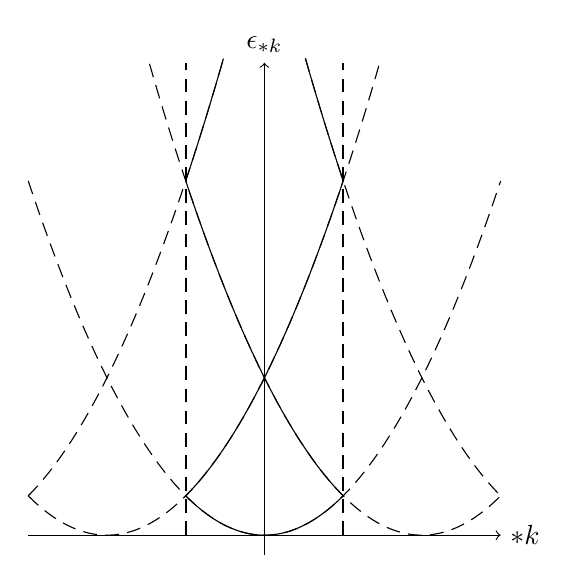
\begin{tikzpicture}
        
            % 动量横轴
            \draw[->] (-3,0) -- (3,0) node[right] {$\vb*{k}$};
            % 动能纵轴
            \draw[->] (0,-0.25) -- (0,6) node[above] {$\epsilon_{\vb*{k}}$};

            % 布里渊区边界
            \draw[dash pattern=on5pt off3pt, thick] (-1, 0) -- (-1, 6);
            \draw[dash pattern=on5pt off3pt, thick] (1, 0) -- (1, 6);
            
            % 画出布里渊区以外的能谱
            
            \draw[dash pattern=on5pt off3pt,samples=50, smooth, domain=-3:1.46] plot(\x,{0.5*((\x+2)*(\x+2))});
            \draw[dash pattern=on5pt off3pt,samples=50, smooth, domain=-3:3] plot(\x,{0.5*((\x)*(\x))});
            \draw[dash pattern=on5pt off3pt,samples=50, smooth, domain=-1.46:3] plot(\x,{0.5*((\x-2)*(\x-2))});
            \draw[dash pattern=on5pt off3pt,samples=50, smooth, domain=0.52:3] plot(\x,{0.5*((\x-4)*(\x-4))});
            \draw[dash pattern=on5pt off3pt,samples=50, smooth, domain=-3:-0.52] plot(\x,{0.5*((\x+4)*(\x+4))});

            % 画出布里渊区内部的$\epsilon_{\vb*{k}}$曲线,以及由于晶格周期性而导致的能谱平移
            \draw[samples=50, smooth, domain=-1:1] plot(\x,{0.5*(\x*\x)});
            \draw[samples=50, smooth, domain=-1:1] plot(\x,{0.5*((\x-2)*(\x-2))});
            \draw[samples=50, smooth, domain=-1:1] plot(\x,{0.5*((\x+2)*(\x+2))});
            \draw[samples=50, smooth, domain=0.52:1] plot(\x,{0.5*((\x-4)*(\x-4))});
            \draw[samples=50, smooth, domain=-1:-0.52] plot(\x,{0.5*((\x+4)*(\x+4))});
    
        \end{tikzpicture}
        
    }
    \subfigure[相互作用打开能隙,形成分离的能带]{
        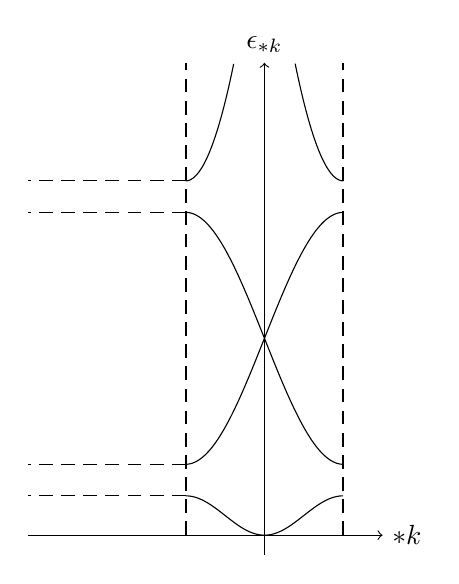
\begin{tikzpicture}
        
            % 动量横轴
            \draw[->] (-3,0) -- (1.5,0) node[right] {$\vb*{k}$};
            % 动能纵轴
            \draw[->] (0,-0.25) -- (0,6) node[above] {$\epsilon_{\vb*{k}}$};

            % 布里渊区边界
            \draw[dash pattern=on5pt off3pt, thick] (-1, 0) -- (-1, 6);
            \draw[dash pattern=on5pt off3pt, thick] (1, 0) -- (1, 6);
            
            % 画出布里渊区内部的$\epsilon_{\vb*{k}}$曲线,以及由于晶格周期性而导致的能谱平移
            \draw[samples=50, smooth, domain=-1:1] plot(\x,{0.25-0.25*cos(3.14*\x r)});
            \draw[samples=50, smooth, domain=-1:1] plot(\x,{2.5+1.6*sin(1.57*\x r)});
            \draw[samples=50, smooth, domain=-1:1] plot(\x,{2.5-1.6*sin(1.57*\x r)});
            \draw[samples=50, smooth, domain=0.39:1] plot(\x,{4.5+4*(\x-1)*(\x-1)});
            \draw[samples=50, smooth, domain=-1:-0.39] plot(\x,{4.5+4*(\x+1)*(\x+1)});

            % 标记能带和带隙
            \foreach \hei in {0.5, 0.9, 4.1, 4.5}
                \draw[dash pattern=on5pt off3pt] (-1,\hei) -- (-3, \hei);
    
        \end{tikzpicture}
        
    }
    \caption{能带结构}
    \label{fig:bloch-energy-band}
\end{figure}

\begin{tikzpicture}
        
    % 动量横轴
    \draw[->] (-4,0) -- (4,0);
    \node[right] at (4, 0) {$k$};

    % 动量零点
    \draw[dash pattern=on5pt off3pt] (0,0.7) -- (0,-0.7);
    
    % 标黑费米球
    \draw[thick] (-1.5,0) -- (1.5,0);

    % 标出费米点
    \node[dot, label=above:$k_\text{F}$] at (1.5, 0) {};
    \node[dot, label=above:$-k_\text{F}$] at (-1.5, 0) {};

\end{tikzpicture}

%%%%%%%%%%%%%%%%%%%%%%%%%%%%%%%%%%%%%%%%%%%%%%%%%%%%%%%%5

The topological order described above has nothing to do with symmetries - their occurrences do not depend on certain symmetries, nor do they break any symmetry.
Nonetheless, there is no guarantee that ordinary symmetric operations always commute with topological operations, so there may be ``interaction'' between symmetries and topological orders, which is denoted by \concept{Symmetry enriched topological order}, or \concept{SET}.
Frequently observed SETs include
\begin{enumerate}
    \item Instrinsic topological order + symmetry protected topological order (SPT)
    \item symmetry fractionalization
    \item symmetry changes state
\end{enumerate}

\concept{Symmetry fractionalization} means topological excitations may not strictly follow the symmetries of the system, as long as trivial excitations composed from them follow the symmetries.
This is quite similar to the relation between $SU(2)$ and $SO(3)$.

Symmetry fractionalization is essential both theoretically and experimentally. It provides a good benchmark between different numerical methods. For example, if different numerical methods give slightly different states but all of them are with the same symmetry fractionalization, we are confident to say they actually give the same result, given that symmetry fractionalization is discrete and is not likely to change with acceptable numerical error.